\documentclass[aspectratio=54,xcolor=dvipsnames]{beamer}
\usetheme{SimpleDarkBlue}

% Packages
\usepackage[utf8]{inputenc}
\usepackage{amsmath, amssymb}
\usepackage{graphicx}
\usepackage{hyperref}
\usepackage{physics}
% \usepackage{siunitx}
% \AtBeginDocument{\RenewCommandCopy\qty\SI}


% Title Information
\title{Computational Electromagnetics Project}
\author{Francesco Fischetti}
\institute{Politecnico di Milano}
\date{\today}

\begin{document}

% Title Slide
\begin{frame}
    \titlepage
\end{frame}

% Outline Slide
\begin{frame}{Outline}
    \tableofcontents
\end{frame}


\section{Recall: Maxwell's Equations}
\begin{frame}{Recall: Maxwell's Equations}
    Maxwell's equations in differential form are given by:
    \begin{align*}
        \nabla \cdot \vec{D} &= \rho \\
        \nabla \cdot \vec{B} &= 0 \\
        \nabla \times \vec{E} &= -\frac{\partial \vec{B}}{\partial t} \\
        \nabla \times \vec{H} &= \vec{J} + \frac{\partial \vec{D}}{\partial t}
    \end{align*}

    \begin{center}
    %\scriptsize
    \begin{tabular}{|c|l|c|}
        \hline
        Symbol & Quantity & Unit \\
        \hline
        $\vec{D}(\vec{r})$ & Electric flux density & $C/m^2$ \\
        $\vec{B}(\vec{r})$ & Magnetic flux density & $T$ \\
        $\vec{E}(\vec{r})$ & Electric field & $V/m$ \\
        $\vec{H}(\vec{r})$ & Magnetic field & $A/m$ \\
        $\vec{J}(\vec{r})$ & Current density & $A/m^2$ \\
        $\rho(\vec{r})$ & Volume charge density & $C/m^3$ \\
        \hline
    \end{tabular}
    %\normalsize
    \end{center}
\end{frame}

\begin{frame}{Recall: Constitutive Relations}
    For a linear and isotropic medium the constitutive relations read
    \begin{align*}
        \vec{D} &= \epsilon \vec{E} \\
        \vec{B} &= \mu \vec{H} \\
        \vec{J} &= \sigma \vec{E}
    \end{align*}
    \vspace{0.5em}
    where
    \begin{center}
    \begin{tabular}{|c|l|c|}
        \hline
        Symbol & Quantity & Unit \\
        \hline
        $\epsilon$ & Dielectric permittivity & $[F/m]$ \\
        $\mu$ & Magnetic permeability & $[H/m]$ \\
        $\sigma$ & Electric conductivity & $[S/m]$ \\
        \hline
    \end{tabular}
    \end{center}
\end{frame}

\section{Problem description and Electromagnetic Field Equations}
\begin{frame}{Problem description}
    Consider 2 infinitely long parallel conductors, with cross sections $\Omega_c$, with $c=1,2$. Each conductor is assumed to have electrical conductivity $\sigma_c$, permittivity $\varepsilon_c$, and magnetic permeability $\mu_c$. The electromagnetic problem becomes two-dimensional with translational symmetry. We assume that the conductors are infinitely long in the $z$-direction.
        \begin{figure}[h]
            \centering
            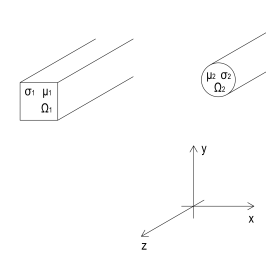
\includegraphics[width=0.35\textwidth]{Images/Conductors_figure.png}
            \caption{Geometry of the two parallel conductors.}
            \label{fig:conductors}
        \end{figure}
\end{frame}

\begin{frame}{The Electromagnetic Field Equations I}
    In multipath eddy current problems where charges and displacement currents are negligible, the steady state time harmonic electromagnetic field is governed by:
    \begin{align}
        \nabla \cdot \tilde{\vec{D}} &= 0 \label{eq:divD} \\
        \nabla \cdot \tilde{\vec{B}} &= 0 \label{eq:divB} \\
        \nabla \times \tilde{\vec{E}} &= - j \omega \tilde{\vec{B}} \label{eq:curlE} \\
        \nabla \times \tilde{\vec{H}} &= \tilde{\vec{J}} \label{eq:curlH}
    \end{align}
    where $j$ is the imaginary unit and $\omega$ is the angular frequency. For the above complex fields, the time dependence is obtained by the substitution:
    \begin{equation*}
        \vec{V}(\vec{r}, t) = \sqrt{2} \cdot \Re \left\{ \tilde{\vec{V}}(\vec{r}) \cdot e^{j \omega t} \right\}
    \end{equation*}
    From now on, we will omit the tilde notation for the complex fields.
\end{frame}

\begin{frame}{The Electromagnetic Field Equations II}
    We introduce the Magnetic Vector Potential (MVP) as
    \begin{equation}
        \vec{B} = \mu \vec{H} = \nabla \times \vec{A}, \qquad \text{ with } \nabla \cdot \vec{A} = 0 \label{eq:divA}
    \end{equation}
    In this case all the variables are constant along $z$ (Figure~\ref{fig:conductors}), and:
    \begin{equation}
        \vec{H} = H_x \vec{e}_x + H_y \vec{e}_y, \qquad
        \vec{J} = J \vec{e}_z, \qquad
        \vec{A} = A \vec{e}_z. \label{ed:2D}
    \end{equation}
    Substituting \eqref{eq:divA} into the Maxwell's equations, we obtain that \eqref{eq:divB} is automatically satisfied, and \eqref{eq:curlH} becomes:
    \begin{equation}
        \nabla \times \left( \frac{1}{\mu} \nabla \times \vec{A} \right) = \vec{J}\label{eq:curlA}
    \end{equation}
    Using \eqref{ed:2D}, we can rewrite \eqref{eq:curlA} as:
    \begin{equation}
        \nabla \cdot \left( \frac{1}{\mu} \nabla A \right) = -J \label{eq:laplacianA}
    \end{equation}
\end{frame}

\begin{frame}{The Electromagnetic Field Equations III}
    The relationship between the electric field $\vec{E}$ and the magnetic vector potential $\vec{A}$ is obtained by substituting equation~\eqref{eq:divA} into equation~\eqref{eq:curlE} and integrating. The result is:
    \begin{equation}
        \vec{E} = -j\omega \vec{A} - \nabla \phi \label{eq:E}
    \end{equation}
    where $\phi$ is the electric scalar potential.
    \newline
    We define:
    \begin{equation}
        \vec{J}_s = - \sigma \nabla \phi, \qquad
        \vec{J}_e = - j \omega \sigma \vec{A},  \qquad 
        \text{so that: } \vec{J} = \vec{J}_e + \vec{J}_s \label{eq:JsJe}
    \end{equation}
    We can also define:
    \begin{equation}
        \vec{A}_s =  \frac{\vec{J}_s}{- j \omega \sigma}
    \end{equation}
    Writing equation~\eqref{eq:JsJe} in scalar form, we have: 
    \begin{equation}
        J = J_e + J_s = - j \omega \sigma A - \sigma \nabla \phi \cdot \vec{e}_z \label{eq:JsJe_scalar}
    \end{equation}
\end{frame}

\begin{frame}{The Electromagnetic Field Equations IV}
    Combining equations~\eqref{eq:laplacianA} and~\eqref{eq:JsJe_scalar}, we obtain the following system of equations:
    \begin{equation}\label{eq:system_equations}
        \left\{
        \begin{aligned}
            \nabla \cdot \left( \frac{1}{\mu} \nabla A \right) - j\omega \sigma A - j\omega \sigma A_s &= 0 
            \\[1em]
            - j\omega \sigma A - j\omega \sigma A_s &= J 
        \end{aligned}
        \right.
    \end{equation}
    The system of equations must be solved subject to appropriate boundary conditions. In these equations, $A$ and $A_s$ are the unknowns, while $J$ is specified in the integral form:
    \begin{equation}
        \int_{\Omega_k} J \, ds = I_k
        \label{eq:current_constraint}
    \end{equation}
    where $I_k$ is the current flowing in conductor $C_k$ of cross-section $\Omega_k$, for $k = 1, \ldots, N$.
\end{frame}

\begin{frame}{The Electromagnetic Field Equations: Remarks}
    \begin{footnotesize}
    \begin{itemize}[]
        \item $J_s$ is the external imposed current density by voltage source, it is a constant. Also $A_s = \frac{J_s}{- j \omega \sigma}$ is a constant.
        \item $J_e = J_e(x,y)$ is the induced current density, it is a function of the magnetic vector potential $A(x,y)$.
        \item $\sigma$ is different from zero only in the conductors.  
    \end{itemize}
    The system of equations~\eqref{eq:system_equations} can be rewritten:
    \begin{subequations}
    \begin{equation}
        \nabla \cdot \left( \frac{1}{\mu_0} \nabla A(x,y) \right)  = 0 \quad \text{in } \Omega \setminus \bigcup_{k \in C} \Omega_k
    \end{equation}
    \begin{equation}
        \left\{
        \begin{aligned}
        \nabla \cdot \left( \frac{1}{\mu_0\mu_{r,k}} \nabla A(x,y) \right) - j\omega \sigma_i A(x,y) - j\omega \sigma_i A_{s,k} &= 0 
        \\[1em]
        - j\omega \sigma_i A(x,y) - j\omega \sigma_i A_{s,k} &= J_i 
        \end{aligned}
        \right.
        \qquad             
        \begin{array}{l}
            \text{in } \Omega_i \\
            \forall k \in C
        \end{array}
    \end{equation}
    \end{subequations}
    \end{footnotesize}
\end{frame}

\section{FEM Formulation}
\begin{frame}{Weak Formulation}
    Considering $\mu$ and $\sigma$ as piecewise constant functions, the weak formulation of~\eqref{eq:system_equations} reads: \\
    Find $A \in H^1(\Omega, \mathbb{C})$ and $A_s \in \mathbb{C}$ such that for all $\phi \in H^1(\Omega, \mathbb{C})$:
    \begin{equation} 
        \int_{\Omega} \left( \frac{1}{\mu} \nabla A \cdot \nabla \phi - j\omega \sigma A \, \phi - j\omega \sigma A_s \, \phi \right) ds = 0
        \label{eq:weak_formulation}
    \end{equation}
    Coupled with:
    \begin{equation}
        \int_{\Omega_k} \left(- j\omega \sigma A - j\omega \sigma A_s \right) ds = \int_{\Omega_k} J \, ds, \quad \forall k \in C
        \label{eq:current_constraint_weak}
    \end{equation}
    Note that the weak formulation is applied only to the first equation of the system~\eqref{eq:system_equations}
\end{frame}

\begin{frame}{Galerkin Method I}
    Consider the finite element space $V_h \subset H^1(\Omega, \mathbb{C})$ spanned by the basis functions $\{\phi_i\}_{i=1}^{N}$, where $N$ is the number of nodes in the mesh. The approximate solution $A_h$ can be expressed as:
    \begin{align*}
        A_h = \sum_{i=1}^{N} A_i \phi_i
    \end{align*}
    Defining the matrices:
    \begin{align*}
        S_{ij} &= \int_{\Omega} \nabla \phi_i \cdot \nabla \phi_j \, ds, \\
        M_{ij} &= \int_{\Omega} \phi_i \phi_j \, ds, \\
    \end{align*}
    And the column vector:
    \begin{align*}
        q_i = \int_{\Omega} \phi_i \, ds, \quad q^1_i = 
    \end{align*}
\end{frame}

\begin{frame}{Galerkin Method II}
    The equation~\eqref{eq:weak_formulation} can be rewritten in matrix form as:
    \begin{equation}
        \left[
        \begin{array}{ccc}
            \frac{1}{\mu} S - j\omega \sigma T & -j\omega \sigma q^1 & -j\omega \sigma q^2 \\
            -j\omega q^{1t} & -j\omega \sigma \abs{\Omega_1} & 0 \\
            -j\omega q^{2t} & 0 & -j\omega \sigma \abs{\Omega_2}
        \end{array}
        \right]
        \left[
        \begin{array}{c}
            \vec{A} \\
            A_{s,1} \\
            A_{s,2}
        \end{array}
        \right]
        =
        \left[
        \begin{array}{c}
            0 \\
            I_1 \\
            I_2
        \end{array}
        \right]
    \end{equation}
\end{frame}

\section{Implementation}
\begin{frame}{Simulation Setup}
    \begin{itemize}
        \item Domain discretization
        \item Boundary conditions
        \item Source excitation
    \end{itemize}
\end{frame}

\begin{frame}{Algorithm Flowchart}
    \begin{center}
        % \includegraphics[width=0.7\textwidth]{flowchart.png}
        \textit{Flowchart image not available.}
    \end{center}
\end{frame}

\section{Results}
\begin{frame}{Simulation Results}
    \begin{itemize}
        \item Field distributions
        \item Convergence analysis
        \item Validation with analytical solutions
    \end{itemize}
    \begin{center}
        % \includegraphics[width=0.6\textwidth]{results.png}
        \textit{Results image not available.}
    \end{center}
\end{frame}

\section{Conclusion}
\begin{frame}{Conclusion}
    \begin{itemize}
        \item Summary of findings
        \item Future work
    \end{itemize}
\end{frame}

% References
\begin{frame}{References}
    \footnotesize
    \begin{thebibliography}{99}
        \bibitem{sadiku} M. N. O. Sadiku, \emph{Numerical Techniques in Electromagnetics}, CRC Press, 2000.
        \bibitem{taflove} A. Taflove, S. C. Hagness, \emph{Computational Electrodynamics: The Finite-Difference Time-Domain Method}, Artech House, 2005.
    \end{thebibliography}
\end{frame}

\end{document}